\chapter{補間}
    \section{IDTFT を用いた有限長信号の補間}
        \label{IDTFT を用いた有限長信号の補間}
        \subsection{動機}
            有限長の離散時間信号(例えば feedforward フィルタの係数)が与えられたとき,その信号を連続時間信号に拡張して,任意の時刻での値を求めたいときがある。
            例えば feedforward フィルタのインパルス応答が離散時間信号として既知であるとき,非整数の時刻に於ける合理的な値を考えたい(これはアップ・サンプリングの為の poly-phase フィルタの係数を計算する方法の一つである)。
        \subsection{方法}
            \label{IDTFT を用いた有限長信号の補間>方法}
            台有界な離散時間信号 $\xd:\integers\to\complexNumbers$ の DTFT を $\XDTFT:\realNumbers\to\complexNumbers$ とする。
            但し引数は正規化角周波数である。
            連続時間信号 $\hat{x}:\realNumbers\to\realNumbers$ を次式で定義する。
            \[ \hat{x}(t)\coloneq\left.\IDTFT{\XDTFT}(n)\right|_{n\to t} = \frac{1}{2\pi}\integrate{-\pi}{\pi}{\XDTFT(\Omega)\exp\parens*{i\Omega t}}{}{\Omega} = \sum_{m=-\infty}^\infty \xd(m)\sinc\pi(t-m) \]
            $\hat{x}$ は全ての離散時刻に於いて $\xd$ と一致する連続関数である。
            これは \ref{標本化定理} に於いて $F_1=1/2$ とした場合の式と同じである。
            \par
            例えば $\xd$ が既知であって,それをある時間 $d\in(0,1)$ だけ仮想的に遅らせた(サンプリング時刻が仮想的に $d$ だけ早まった)離散時間信号は $n\in\integers\mapsto\hat{x}(n-d)$ である。
            殆ど自明なことだが,この信号の DTFT の絶対値は $\xd$ のそれと等しい。
        \subsection{数値例}
            \label{IDTFT を用いた有限長信号の補間>数値例}
            $N=33,\;\alpha=0.4$ とし,有限長の離散時間信号 $h:\integers\to\realNumbers$ を次式で定義する。
            これは視覚的な解り易さから \cite{learn_sp_from_basic} 式 (8.41) から流用したものである。
            \[
                h(n) = \begin{cases}
                    \alpha & (n=(N-1)/2) \\
                    \alpha\sinc{\parens*{(N-1)/2-\pi}\alpha\pi} & (n\in\{0,1,2,\dots,N-1\}\setminus\{(N-1)/2\}) \\
                    0 & (\text{otherwise})
                \end{cases}
            \]
            次の図は $h$ とその DTFT である。
            \begin{figure}[H]
                \centering
                \begin{minipage}{0.49\hsize}
                    \centering
                    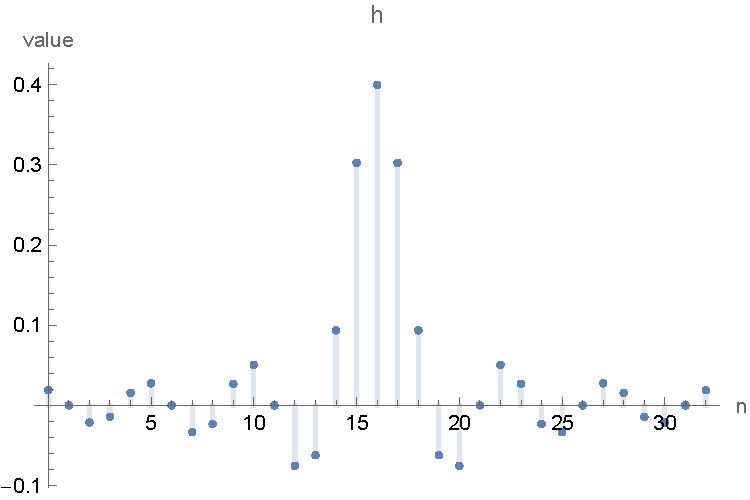
\includegraphics[keepaspectratio, scale=0.69]
                    {\currfiledir/calc/Interpolation_with_IDTFT/h.pdf}
                    \caption{$h$}
                \end{minipage}
                \begin{minipage}{0.49\hsize}
                    \centering
                    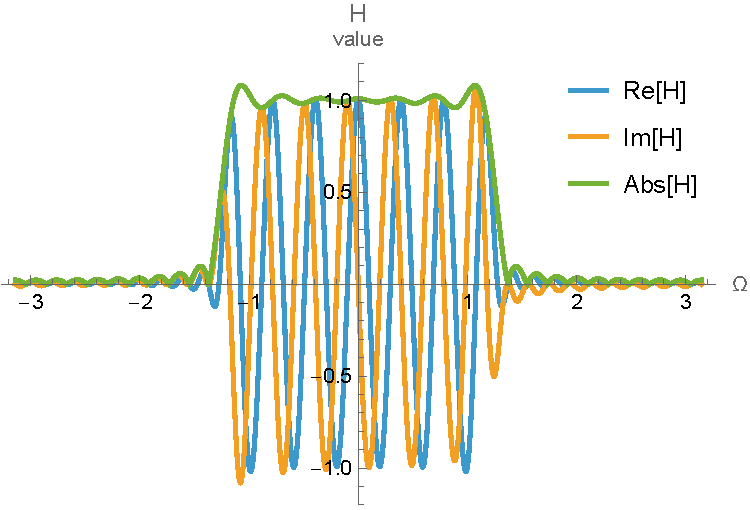
\includegraphics[keepaspectratio, scale=0.69]
                    {\currfiledir/calc/Interpolation_with_IDTFT/DTFT_of_h.pdf}
                    \caption{$h$ の DTFT。横軸は正規化角周波数}
                \end{minipage}
            \end{figure}
            これを前小節の方法で実時間信号に拡張したものを $\tilde{h}$ とする。
            \cref{fig:元の信号と IDTFT による連続時間補間信号} は $h$ と $\tilde{h}$ を重ねて描いたものである。
            \par
            新たな離散時間信号 $h^\dagger:(d,n)\in\realNumbers\times\integers\mapsto\tilde{h}(n-d)$ を定義する。
            $h^\dagger$ は $h$ を仮想的に $d$ だけ遅らせたものである。
            図 \cref{fig:元の信号と IDTFT による実数時間遅延離散時間信号} 2 通りの $d$ について $h^\dagger$ を描いたものである。
            \begin{figure}[H]
                \centering
                \begin{minipage}{0.49\hsize}
                    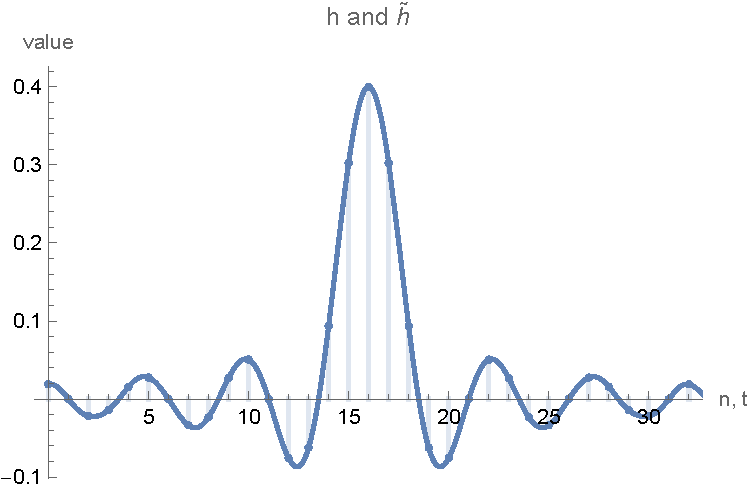
\includegraphics[keepaspectratio, scale=0.69]
                    {\currfiledir/calc/Interpolation_with_IDTFT/h_and_h_tilde.pdf}
                    \caption{$h$ と $\tilde{h}$}
                    \label{fig:元の信号と IDTFT による連続時間補間信号}
                \end{minipage}
                \begin{minipage}{0.49\hsize}
                    \centering
                    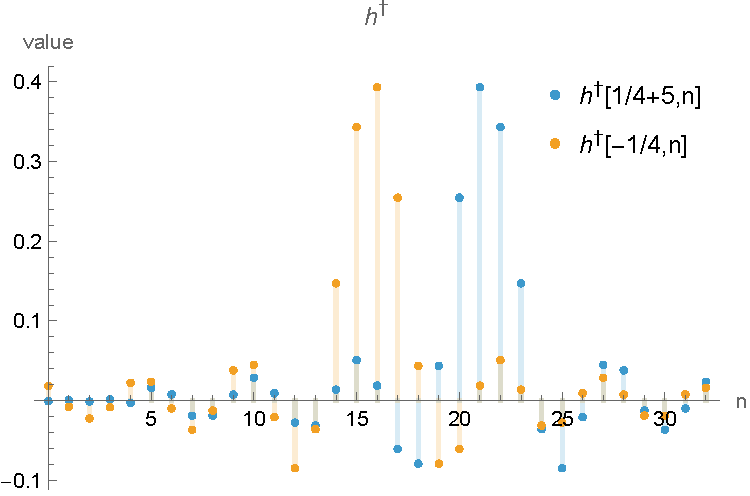
\includegraphics[keepaspectratio, scale=0.69]
                    {\currfiledir/calc/Interpolation_with_IDTFT/h_dag.pdf}
                    \caption{$h^\dagger,\quad d=-0.25,\;0.75$}
                    \label{fig:元の信号と IDTFT による実数時間遅延離散時間信号}
                \end{minipage}
            \end{figure}
            この数値例を計算した Mathematica notebook が下記のファイル名で保存されている。
            Git リポジトリ内でファイル名検索すれば発見できるであろう。
            notebook 中では前記 $N$ が \inlineCode{N_tp} となっている。\newline
            \href{\currfiledir/calc/Interpolation_with_IDTFT/Interpolation_with_IDTFT.nb}{\escapeUnderscore{Interpolation_with_IDTFT.nb}}\newline
        \subsection{等間隔補間信号の周波数スペクトラム}
            \newcommand*{\Xdn}{X_\text{d,n}}
            \newcommand*{\Ydn}{Y_\text{d,n}}
            \ref{IDTFT を用いた有限長信号の補間>方法} の方法で等間隔に補間され $L\;(\in\naturalNumbers,L\geq 2)$ 倍のサンプル周波数を持つ新たな信号の周波数スペクトラムの性質を述べる。
            \begin{shadebox}
                $L$ を 2 以上の自然数とする。
                サンプル周期 $\Ts>0$ の離散時間信号 $\xd:\integers\to\complexNumbers$ を \ref{IDTFT を用いた有限長信号の補間>方法} の方法で等間隔に補間し,サンプル周期 $\Ts/L$ となった離散時間信号を $\yd$ とする。
                但し $\xd,\;\yd$ 両方のサンプリング時刻が 0 を含むものとする。
                $\XDTFT,\;\YDTFT$ を $\xd,\;\yd$ の DTFT とする。
                $\omega\in\realNumbers$ について次式が成り立つ。
                \[ \YDTFT(\omega) = L\sum_{n=-\infty}^\infty \XDTFT\parens*{\omega-n\frac{2\pi L}{\Ts}}\uBox\parens*{\frac{\Ts}{2\pi}\parens*{\omega-\frac{2\pi L}{\Ts}n}} \tag{1} \]
                元のサンプル周期に於ける第 1 Nyquist 領域の外側で $\XDTFT$ を 0 としたものが, $\Ts/(2\pi L)$ 周期拡張されている。
                \par
                $\Xdn,\;\Ydn$ を $\xd,\;\yd$ の DTFT であって引数が正規化角周波数 $\Omega\in\realNumbers$ であるものとする(前者と後者の正規化角周波数はスケールが異なる。それぞれ $\omega\Ts,\;\omega\Ts/L$)。
                これを用いて式 (1) を書き直すと次式である。
                \[ \Ydn(\Omega) = L\sum_{n=-\infty}^\infty \Xdn\parens*{L(\Omega-2\pi n)}\uBox\parens*{\frac{L}{2\pi}\parens*{\Omega-2\pi n}} \tag{2} \]
                元のサンプル周期に於ける第 1 Nyquist 領域の外側で $\Xdn$ を 0 とした後に角周波数軸方向に $1/L$ 倍に縮めたものが $2\pi$ 周期拡張されている。
            \end{shadebox}
            \begin{proof}
                \begin{align*}
                    \yd(n) &= \left.\xd(n)\right|_{n\to n/L} = \frac{\Ts}{2\pi}\integrate{-\pi/\Ts}{\pi/\Ts}{\XDTFT(\omega)\exp(i\omega n\Ts/L)}{}{\omega} \\
                    \YDTFT(\omega) &= \sum_{n=-\infty}^\infty \yd(n)\exp(-i\omega n\Ts/L) \tag{3} \\
                    &= \sum_{n=-\infty}^\infty \frac{\Ts}{2\pi}\integrate{-\pi/\Ts}{\pi/\Ts}{\XDTFT(\tilde{\omega})\exp(i\tilde{\omega} n\Ts/L)}{}{\tilde{\omega}}\exp(-i\omega n\Ts/L) \\
                    &= \frac{\Ts}{2\pi}\integrate{-\pi/\Ts}{\pi/\Ts}{\XDTFT(\tilde{\omega})\sum_{n=-\infty}^\infty\exp(i(\tilde{\omega}-\omega)n\Ts/L)}{}{\tilde{\omega}} \\
                    &= \frac{\Ts}{2\pi}\integrate{-\pi/\Ts}{\pi/\Ts}{\XDTFT(\tilde{\omega})\frac{2\pi L}{\Ts}\sum_{n=-\infty}^\infty\delta(\tilde{\omega}-\omega-2\pi Ln/\Ts)}{}{\tilde{\omega}} \quad (\text{\ref{定数関数1のDTFT}} を用いた) \\
                    &= L\sum_{n=-\infty}^\infty\integrate{-\pi/\Ts}{\pi/\Ts}{\XDTFT(\tilde{\omega})\delta(\tilde{\omega}-\omega-2\pi Ln/\Ts)}{}{\tilde{\omega}}
                \end{align*}
                この式の評価には注意を要する。
                式 (3) より $\YDTFT$ が $2\pi L/\Ts$ 周期関数であることが解るから,区間 $[-\pi L/\Ts,\pi L/\Ts]$ に於ける式を構築した後に $2\pi L/\Ts$ 周期拡張すればよい。
                \par
                まず $\omega\in[-\pi L/\Ts,\pi L/\Ts]\setminus[-\pi/\Ts,\pi/\Ts]$ のとき,$n$ がどうであっても $\omega+2\pi Ln/\Ts$ は $[-\pi/\Ts,\pi/\Ts]$ に属さないから $\YDTFT(\omega)=0$ である。
                次に $\omega\in[-\pi/\Ts,\pi/\Ts]$ のとき,$\omega+2\pi Ln/\Ts$ は $n=0$ のとき,かつそのときに限り $[-\pi/\Ts,\pi/\Ts]$ に属すから $\YDTFT(\omega)=\XDTFT(\omega)$ である。
                以上 2 つから,区間 $[-\pi L/\Ts,\pi L/\Ts]$ に於いては $\YDTFT(\omega) = \XDTFT(\omega)\uBox(\omega\Ts/(2\pi))$ である。
                これを $2\pi L/\Ts$ 周期拡張すれば式 (1) が得られる。
                \par
                式 (1) に於いて $\omega$ を $\Omega/\Ts$ で書き換え,関係式 $\XDTFT(\Omega/\Ts) = \Xdn(\Omega)$ を用いると式 (2) が得られる。
            \end{proof}
            \subsubsection{数値例}
                \ref{IDTFT を用いた有限長信号の補間>数値例} の $h$ を $4$ 倍に補間した信号 $h_\text{itp}$ とその DTFT の絶対値を次の図に示す。
                \begin{figure}[H]
                    \centering
                    \begin{minipage}{0.49\hsize}
                        \centering
                        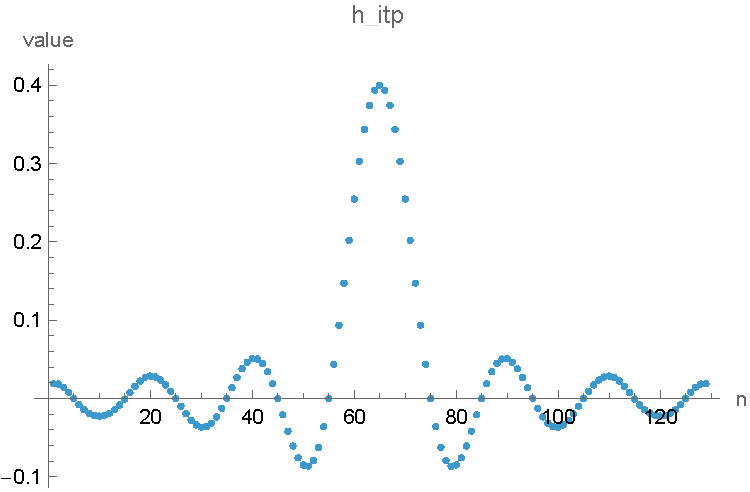
\includegraphics[keepaspectratio, scale=0.69]
                        {\currfiledir/calc/Interpolation_with_IDTFT/h_itp.pdf}
                        \caption{$h_\text{itp}$}
                    \end{minipage}
                    \begin{minipage}{0.49\hsize}
                        \centering
                        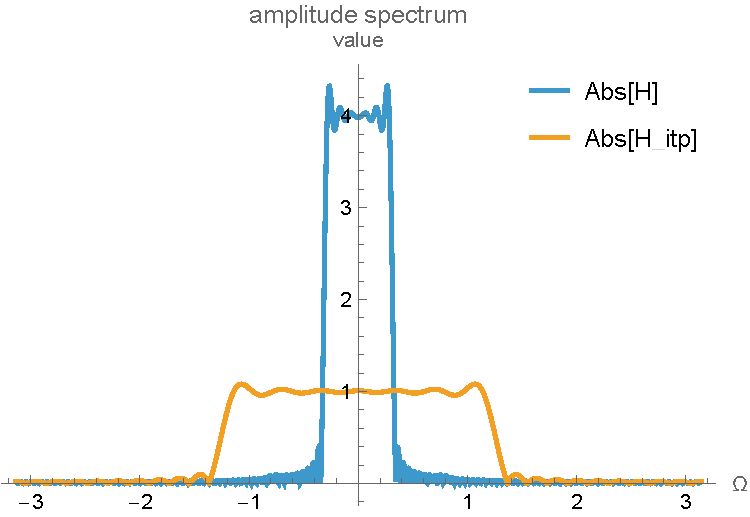
\includegraphics[keepaspectratio, scale=0.69]
                        {\currfiledir/calc/Interpolation_with_IDTFT/abs_of_H_and_H_itp.pdf}
                        \caption{$h,\;h_\text{itp}$ の DTFT。横軸は正規化角周波数}
                    \end{minipage}
                \end{figure}
    \section{IDFT を用いた周期信号の補間}
        \subsection{動機}
            周期的な離散時間信号が与えられたとき,その信号を連続時間信号に拡張して,任意の時刻での値を求めたいときがある。
            例えば 2 次元平面上で閉曲線を描く粗い点列が与えられたとき,より細かく合理的な点列を考えたい。
            \par
            これは \ref{IDTFT を用いた有限長信号の補間} によっても可能(元の信号の離散時刻の上下端点をそれぞれ 1 つ分巡回的に拡張すればよい)であるが,補間対象の信号の台の長さ $N$ に対して計算量は $O(N^2)$ である。
            一方で,以下で述べる方法は DFT と IDFT 、および元の信号の周期に比例する計算量の操作で実行可能であり,DFT, IDFT は FFT を活用して高速に計算できるから,計算量は $O(N\log_2 N)$ である。
            ただし信号の周期 $N$ は奇数に限られ,FFT に最も都合の良い 2 の冪乗ではない(参考情報として $N$ が偶数のときに無理矢理適用して失敗した結果を \ref{N が偶数のときに無理矢理適用した結果} に記した)。
        \subsection{方法}
            \label{IDFT を用いた周期信号の補間>方法}
            \newcommand*{\Xtilded}{\tilde{X}_\text{d}}
            $N$ を奇数の自然数とする。$N$ 周期離散時間信号 $\xd:\integers\to\complexNumbers$ の DFT を $\XDTFT$ とする。
            連続時間信号 $\hat{x}$ を次式で定義する。
            \[ \hat{x}(t) \coloneq \frac{1}{\sqrt{N}}\sum_{k=-(N-1)/2}^{(N-1)/2}\XDTFT(k\%N)\exp i2\pi\frac{1}{N}kt \tag{1} \]
            これは $t\in\integers$ のとき $\xd(t)$ と一致する(性質 1)。
            特に $n\in\integers,\;\Delta t\in[0,1)$ であるとき次式が成り立つ(性質 2)。
            \begin{gather}
                \hat{x}(n+\Delta t) = \parens*{\exp i\pi\frac{1-N}{N}n}\IDFT{\Xtilded}(n) \label{IDFT を用いた周期信号の補間>公式}\\
                \text{where} \quad \Xtilded:k\in\integers\mapsto\XDTFT\parens*{\parens*{k-\frac{N-1}{2}}\%N}\bracks*{\exp i2\pi\frac{1}{N}\parens*{k-\frac{N-1}{2}}\Delta t} \nonumber
            \end{gather}
            $\Xtilded(k)\;(k=0,1,\dots,N-1)$ は $O(N)$ の計算量で用意できる。
            IDFT の部分は FFT を用いて(データ数が奇数なので亜種を使う)高速に計算できる。
        \subsection{式 (1) を得る発想}
            一見すると,次の式に於いて単純に $n$ を $t$ に置き換えれば上手くいくように思える。
            \[ \xd(n) = \IDFT{\XDTFT}(n) = \frac{1}{\sqrt{N}}\sum_{k=0}^{N-1}\XDTFT(k)\exp\parens*{i2\pi\frac{1}{N}kn} \]
            しかしこれは失敗する。
            例えば $\xd$ が実数値信号であるとき $\XDTFT$ は Hermite 対称である ($\XDTFT(-k)=\XDTFT(N-k)=\conj{\XDTFT(k)}$)。
            $t=n+\Delta t,\;n=\floor{t},\;\Delta t\in[0,1)$ とすると $\xd(t)$ は $k\mapsto\XDTFT(k)\exp i2\pi k\Delta t/N$ の IDFT であるが,これは実数値ではなく,補間の結果として受け入れられない。
            期待通りの結果を得るには \ref{IDTFT を用いた有限長信号の補間>方法} のように総和の範囲を正負対称にし,$\XDTFT$ に手を加えた結果を少なくとも Hermite 対称にする必要がある。
        \subsection{性質 1 の導出}
            \begin{proof}
                \quad\par
                $t = n\in\integers$ とする。
                \begin{align*}
                    \hat{x}(t) &= \hat{x}(n) = \frac{1}{\sqrt{N}}\sum_{k=-(N-1)/2}^{(N-1)/2}\XDTFT(k\%N)\exp i2\pi\frac{1}{N}kn \\
                    &= \frac{1}{\sqrt{N}}\sum_{k=0}^{N-1}\XDTFT((k-(N-1)/2)\%N)\exp i2\pi\frac{1}{N}(k-(N-1)/2)n \\
                    &= \frac{1}{\sqrt{N}}\sum_{k=0}^{N-1}\XDTFT((k-(N-1)/2)\%N)\exp i2\pi\frac{1}{N}[(k-(N-1)/2)\%N]n \\
                    &= \frac{1}{\sqrt{N}}\sum_{k=0}^{N-1}\XDTFT(k)\exp i2\pi\frac{1}{N}kn = \xd(n)
                \end{align*}
            \end{proof}
        \subsection{性質 2 の導出}
            \begin{proof}
                \begin{align*}
                    \hat{x}(n+\Delta t) &= \frac{1}{\sqrt{N}}\sum_{k=-(N-1)/2}^{(N-1)/2}\XDTFT(k\%N)\exp i2\pi\frac{1}{N}k(n+\Delta t) \\
                    &= \frac{1}{\sqrt{N}}\sum_{k=-(N-1)/2}^{(N-1)/2}\XDTFT(k\%N)\parens*{\exp i2\pi\frac{1}{N}k\Delta t}\exp i2\pi\frac{1}{N}kn \\
                    &= \frac{1}{\sqrt{N}}\sum_{k=0}^{N-1}\XDTFT\parens*{\parens*{k-\frac{N-1}{2}}\%N}\bracks*{\exp i2\pi\frac{1}{N}\parens*{k-\frac{N-1}{2}}\Delta t}\exp i2\pi\frac{1}{N}\parens*{k-\frac{N-1}{2}}n \\
                    &= \parens*{\exp i\pi\frac{1-N}{N}n}\frac{1}{\sqrt{N}}\sum_{k=0}^{N-1}\XDTFT\parens*{\parens*{k-\frac{N-1}{2}}\%N}\bracks*{\exp i2\pi\frac{1}{N}\parens*{k-\frac{N-1}{2}}\Delta t}\exp i2\pi\frac{1}{N}n \\
                    &= \parens*{\exp i\pi\frac{1-N}{N}n}\IDFT{\Xtilded}(n)
                \end{align*}
            \end{proof}
        \subsection{数値例}
            \label{IDFT を用いた周期信号の補間>数値例}
            次式で定義される 2 次元平面上の閉曲線 $C:r(t)\;;t:0\to 1$ を $1/N_\text{pt} \coloneq 1/33$ 間隔で $t=0$ から $(N_\text{pt}-1)/N_\text{pt}$ まで標本化した離散座標周期列を $r_\text{d}:\integers\to\realNumbers^2$ とする。
            \[
                r: t\in\realNumbers\mapsto\begin{bmatrix}
                    (1+(\cos 4\pi t)/2+(\cos 14\pi t)/8)\cos 2\pi t \\
                    (1+(\sin 5\pi t^{3/2})/2+(\sin 23\pi t)/8)\sin 2\pi t
                \end{bmatrix}
            \]
            \begin{figure}[H]
                \centering
                \begin{minipage}{0.49\hsize}
                    \centering
                    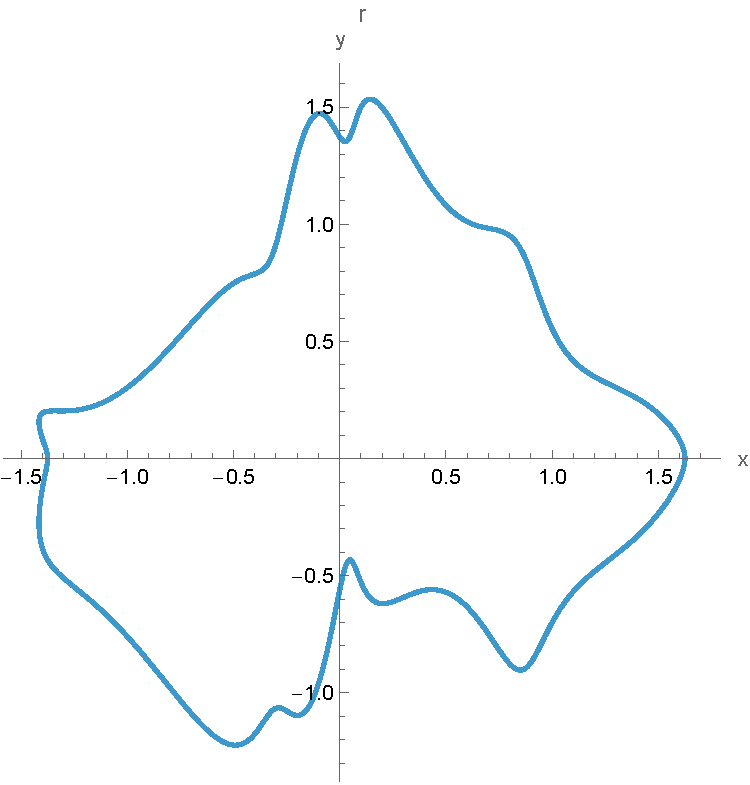
\includegraphics[keepaspectratio, scale=0.69]
                    {\currfiledir/calc/Interpolation_with_IDFT/interpolation_with_IDFT_N=odd_x=2D_closed_curve/r.pdf}
                    \caption{$r$}
                \end{minipage}
                \begin{minipage}{0.49\hsize}
                    \centering
                    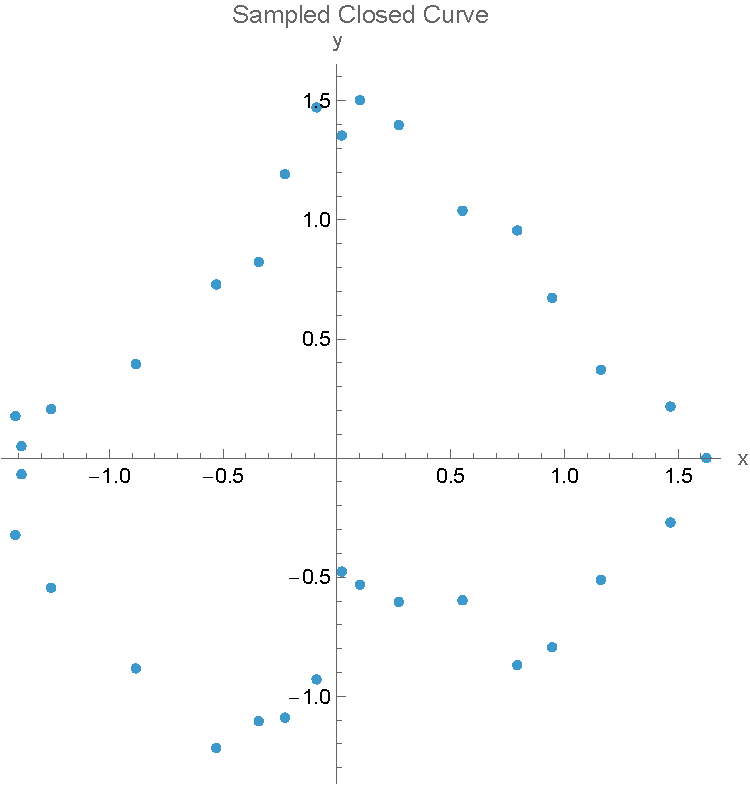
\includegraphics[keepaspectratio, scale=0.69]
                    {\currfiledir/calc/Interpolation_with_IDFT/interpolation_with_IDFT_N=odd_x=2D_closed_curve/r_d.pdf}
                    \caption{$r_\text{d}$}
                \end{minipage}
            \end{figure}
            次の図はこれを IDFT を使う方法で 4 倍に補間した離散座標周期列 $r_\text{itp}$ である。
            \begin{figure}[H]
                \centering
                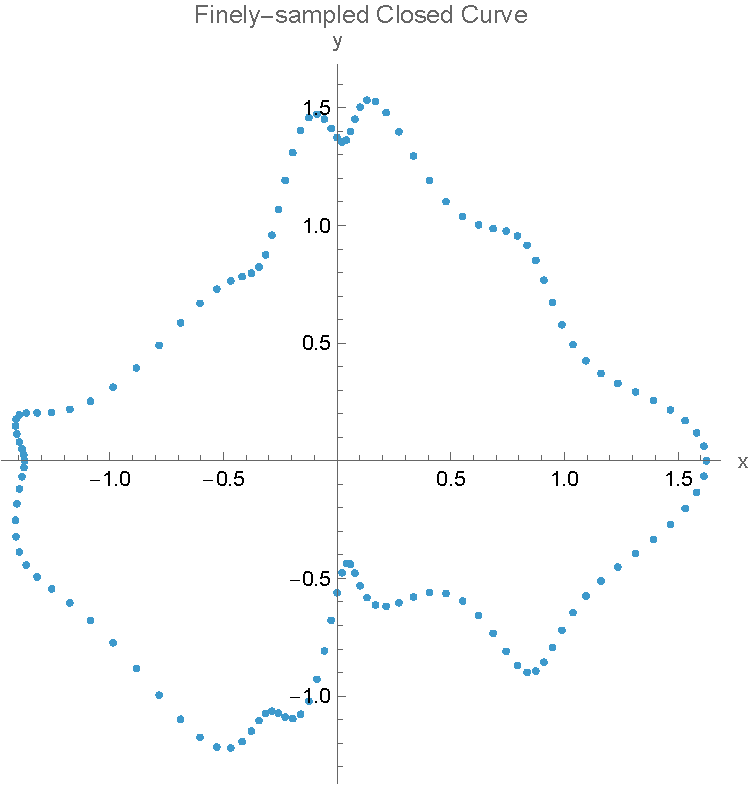
\includegraphics[keepaspectratio, scale=0.69]
                {\currfiledir/calc/Interpolation_with_IDFT/interpolation_with_IDFT_N=odd_x=2D_closed_curve/r_itp.pdf}
                \caption{$r_\text{itp}$}
            \end{figure}
            この数値例を計算した Mathematica notebook が下記のファイル名で保存されている。
            Git リポジトリ内でファイル名検索すれば発見できるであろう。
            notebook 中では実装の都合上,前記 $r$ の成分を $x,y$ として分けて扱っている。\newline
            \begin{itemize}
                \item \href{\currfiledir/calc/Interpolation_with_IDFT/interpolation_with_IDFT_N=odd_x=2D_closed_curve/interpolation_with_IDFT_N=odd_x=2D_closed_curve.nb}{\escapeUnderscore{interpolation_with_IDFT_N=odd_x=2D_closed_curve.nb}}:前記の数値例
                \item \href{\currfiledir/calc/Interpolation_with_IDFT/interpolation_with_IDFT_N=odd/interpolation_with_IDFT_N=odd.nb}{\escapeUnderscore{interpolation_with_IDFT_N=odd.nb}}:上記の数値例の前身。$x$ 成分のみを扱っている。
            \end{itemize}
        \subsection{N が偶数のときに無理矢理適用した結果}
            \label{N が偶数のときに無理矢理適用した結果}
            式 \eqref{IDFT を用いた周期信号の補間>公式} に於いて仮に $N$ を偶数とした場合の結果が次の Mathematica notebook に記されている。
            大雑把にそれらしい結果が得られているが,補間結果が不自然に波打っている。\newline
            \href{\currfiledir/calc/Interpolation_with_IDFT/interpolation_with_IDFT_N=even/interpolation_with_IDFT_N=even.nb}{\escapeUnderscore{interpolation_with_IDFT_N=even.nb}}
        \subsection{等間隔補間信号の周波数スペクトラム}
            \ref{IDFT を用いた周期信号の補間>方法} の方法で等間隔に補間され $L\;(\in\naturalNumbers,L\geq 2)$ 倍の周期を持つ新たな信号の周波数スペクトラムの性質を述べる。
            $L$ に偶奇の制約はない。
            \begin{shadebox}
                $L$ を 2 以上の自然数,$N$ を奇数の自然数とする。
                周期 $N$ の離散時間信号 $\xd:\integers\to\complexNumbers$ を \ref{IDFT を用いた周期信号の補間>方法} の方法で等間隔に補間し,周期 $LN$ となった離散時間信号を $\yd$ とする。
                但し $\yd(0) = \xd(0)$ とする。
                $\XDTFT,\YDTFT$ を $\xd,\yd$ の DFT とする。$k\in\integers$ について次式が成り立つ。
                \[ \YDTFT(k) = \sqrt{L}\sum_{n=-\infty}^{\infty}X(k-nLN)\uBox\parens*{\frac{k-nLN}{N-1}} \]
                これは $\XDTFT$ を $\sqrt{L}$ 倍して台を $\{-(N-1)/2,-(N-1)/2+1,\dots,(N-1)/2\}$ に制限したものを $LN$ 間隔で無限に並べ,隙間に 0 を置いたものと等しい。
            \end{shadebox}
            \begin{proof}
                \quad\par
                DFT の性質から $\YDTFT$ が $LN$ 周期関数であることが解る。
                そこで,まず集合 $I\coloneq\{-\floor{(LN-1)/2},\;-\floor{(LN-1)/2}+1,\;\dots,\;\floor{(LN-1)/2}-1\}$ ($LN$ の偶奇に関係なく適切な集合であることに注意すべし)上で $\YDTFT$ を評価し,それを $LN$ 周期拡張する。
                $I$ に於いては次式が成り立つ。
                \begin{align*}
                    \YDTFT(k) &= \frac{1}{\sqrt{LN}}\sum_{n=0}^{LN-1}\yd(n)\exp\parens*{-i\frac{2\pi}{LN}kn} \\
                    &= \frac{1}{\sqrt{LN}}\sum_{n=0}^{LN-1}\parens*{\frac{1}{\sqrt{N}}\sum_{l=-(N-1)/2}^{(N-1)/2}X(l)\exp\parens*{i\frac{2\pi}{N}l\frac{n}{L}}}\exp\parens*{-i\frac{2\pi}{LN}kn} \\
                    &= \frac{1}{N\sqrt{L}}\sum_{l=-(N-1)/2}^{(N-1)/2}X(l)\sum_{n=0}^{LN-1}\exp\parens*{i\frac{2\pi}{LN}(l-k)n} = \frac{1}{N\sqrt{L}}\sum_{l=-(N-1)/2}^{(N-1)/2}X(l)LN\delta(l-k) \\
                    &= \begin{cases}
                        \sqrt{L}X(k) & (\abs{k}\leq (N-1)/2) \\
                        0 & (k\in I\land\abs{k}>(N-1)/2)
                    \end{cases}
                \end{align*}
                これを $LN$ 周期拡張すれば定理の主張が従う。
            \end{proof}
            \subsubsection{数値例}
                \ref{IDFT を用いた周期信号の補間>数値例} の $x$ 成分について前述の性質を確認する。
                次の図はそれぞれ $\xd$ と $\abs{\XDTFT}$ である。
                \begin{figure}[H]
                    \centering
                    \begin{minipage}{0.49\hsize}
                        \centering
                        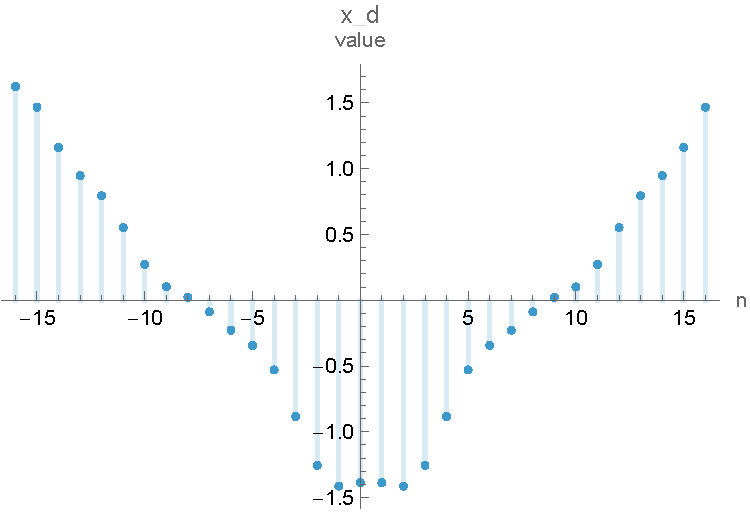
\includegraphics[keepaspectratio, scale=0.69]
                        {\currfiledir/calc/Interpolation_with_IDFT/interpolation_with_IDFT_N=odd/x_d.pdf}
                        \caption{$\xd$}
                    \end{minipage}
                    \begin{minipage}{0.49\hsize}
                        \centering
                        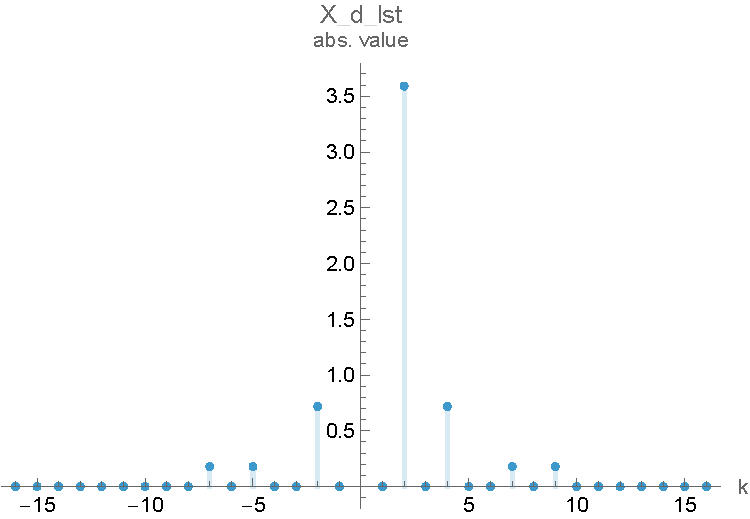
\includegraphics[keepaspectratio, scale=0.69]
                        {\currfiledir/calc/Interpolation_with_IDFT/interpolation_with_IDFT_N=odd/abs_X_d.pdf}
                        \caption{$\abs{\XDTFT}$}
                    \end{minipage}
                \end{figure}
                $\xd$ を 4 倍に補間した信号 $\yd$ とその DTFT $\YDTFT$ の絶対値を次の図に示す。
                \begin{figure}[H]
                    \centering
                    \begin{minipage}{0.49\hsize}
                        \centering
                        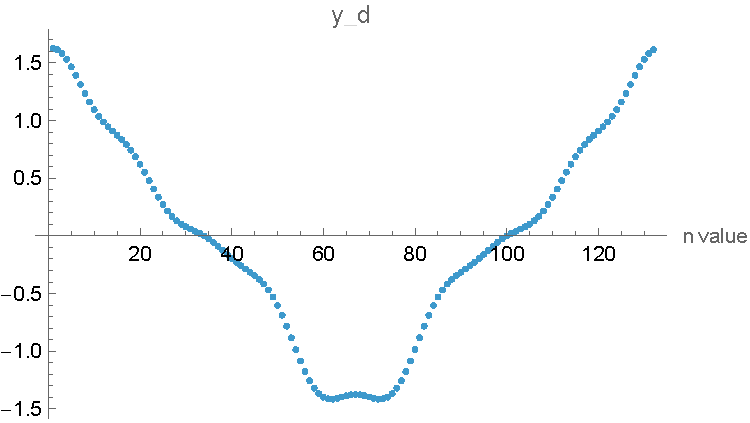
\includegraphics[keepaspectratio, scale=0.69]
                        {\currfiledir/calc/Interpolation_with_IDFT/interpolation_with_IDFT_N=odd/y_d.pdf}
                        \caption{$\yd$}
                    \end{minipage}
                    \begin{minipage}{0.49\hsize}
                        \centering
                        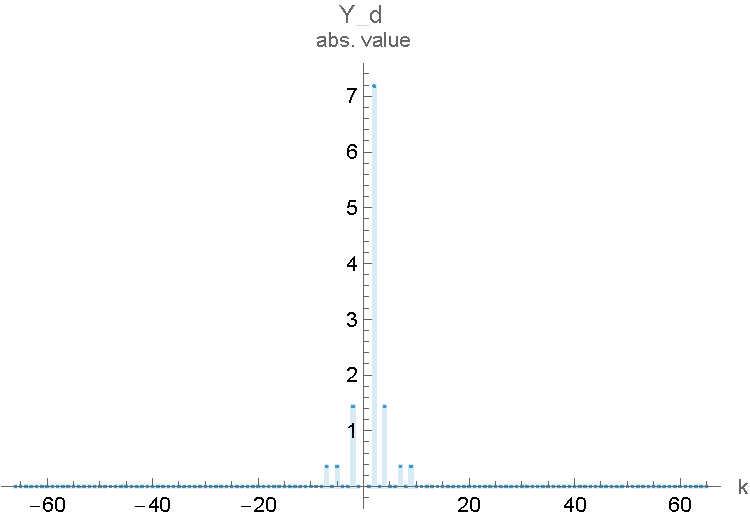
\includegraphics[keepaspectratio, scale=0.69]
                        {\currfiledir/calc/Interpolation_with_IDFT/interpolation_with_IDFT_N=odd/abs_Y_d.pdf}
                        \caption{$\abs{\YDTFT}$}
                    \end{minipage}
                \end{figure}